% Chapter 1

\chapter{Introduction and Literature Survey} % Write in your own chapter title
\label{Chapter1}
\lhead{Chapter 1. \emph{Introduction and Literature Survey}} % Write in your own chapter title to set the page header

In this work, we analyse the problem of passive geolocation of a moving transmitter, using
a stationary array of receivers. We suggest a one-step algorithm for estimating the position and velocity of the transmitter based on one sampling interval. The performance of this algorithm is analyzed, tested using Monte-Carlo simulations and compared to the performance of conventional methods.\\

The signal processing problem of passive transmitter geolocation has been greatly discussed since World War I. It has both civil and military related applications. Among the military applications we can mention passive geolocation of communication systems, radars, GPS blockers and passive low-signature geolocation of air-planes. Among the civil applications we can mention navigation. The extensive use of cellular telephony these days has increased the popularity of this field, and geolocation of cellular phone users is one of the major civil application nowadays, for focused advertising, network load monitoring and enhanced emergency services. The wireless enhanced 911 (E911) review by Zagami et al.\cite{zagami} is one example to the implementation of passive geolocation methods. The wide spread and high density of Wi-Fi networks in highly populated cities nowdays, can serve passive geolocation methods for nevigation inside buildings, or where is no GPS reception. In \cite{wifi} a method for geolocation inside buildings using the Wi-Fi signal strength is presented.\\

Unlike active localization systems such as radar or sonar, that transmit a known signal and process the signal after it was returned from the target, in passive gelocation systems the transmitted signal is usually unknown. Known signals scenarios include, for example, beacon tracking, where a system transmits a known signal in order to be tracked, and scenarios in which there is a communication system that has a known training sequence. In scenarios in which the transmitted signal is known, better performance and lower algorithm complexity can be achieved.\\

While exploring passive geolocation methods, two main approaches can be found: two-step methods and one-step methods. Many two-step methods for passive transmitter geolocation have been suggested in the past \cite {musicki,musicki_kaune_koch,torrieri, chan_jardine, chan_towers, haworth, ho_chan,ho_xu}. The two-step methods first estimate parameters characterizing the signal in each receiver, or in each pair of receivers, and then use these estimated parameters to estimate the location of the transmitter. One step methods were thoroughly discussed in literature and are considered, in general, the classical passive geolocation methods. Two step methods were very popular in the past, and also today, because the parameters characterizing the signals, such as time of arrival, frequency of arrival, signal strength etc., could have been extracted using simple analog components, and because sending the extracted parameters from all the receivers to a central processing station required low-bandwidth communication that was available in the past. Obviously, due the incomplete data used in each receiver or pair of receivers and over-parametrization, two-step methods are sub-optimal.  Recently, one-step methods \cite{dpd,dpd_nb,dop_dpd_nb,dop_dpd_wb} have been suggested and shown to have greater results than the one-step methods. The one-step methods use the sampled signals collected at each of the receivers to simultaneously estimate the position of the transmitter. High frequency digital samplers and high-bandwidth communication systems that exist today, make it possible to employ the one-step methods.\\

Although geolocation of a stationary transmitter by moving receivers has been discussed thoroughly in the literature, the problem of geolocating a moving transmitter has been less discussed. The problem of geolocating a moving transmitter shows greater complexity than geolocating a stationary transmitter, because both the position and velocity of the transmitter are unknown and need to be estimated.\\

In this work, we employ the concepts of the one-step methods for passive geolocation of a moving transmitter. \\

Along this work, we present only the two-dimensional scenario, where the position and velocity of the transmitter lie on a two-dimensional plane. It is simpler to demonstrate the principles of geolocation using the two-dimensional scenarios, and the two-dimensional scenario can be easily expanded to the three-dimensional scenario. Although many applications, such as passive air-plane geolocation, are in-fact three-dimensional scenarios, in many other applications, such as mobile phone geolocation, the plane on which the transmitter could be found is usually known.

In the following chapter, we introduce several two-step and one-step methods suggested for passive geolocation of a stationary transmitter based on delay and doppler.
The two-steps methods we introduce are TOA, TDOA, FOA and FDOA, while the one-step methods introduced are DPD and its derivatives.\\
At the last section of this chapter, we introduce the outline for our work.

\section{Two-Step Localization Methods}
\subsection{Extracting TDOA and FDOA measurements}
The first step in time and frequency shifts based two-step methods is estimating the time and frequency shifts between the received signal and another signal \cite{stein, knapp_carter}. Depending on the method, the estimation can be performed between each pair of receivers, between all the receivers and a reference receiver, or between each receiver and a known reference signal, in the case where the transmitted signal is known.\\

The ML estimation of the delay and Doppler suggested by S. Stein \cite{stein} presents the following formulation.
Two noisy signals $y_1(t)$ and $y_2(t)$, observed over the interval $(0,T)$, are assumed to contain a common signal $x(t)$, appearing in $y_2(t)$ with a relative complex gain factor $\alpha$, at a differential delay $\tau$ and with a frequency offset $\nu$, all unknown. In complex envelope notation:
\begin{eqnarray}
y_1(t) &=& x(t)+n_1(t)\\
y_2(t) &=& \alpha x(t+\tau)e^{2 \pi j \nu (t+\tau)} + n_2(t) \nonumber
\end{eqnarray}

For spectrally flat noise, the ML suggested estimator is shown to be the maximum of the complex cross-ambiguity function.
\begin{equation}
R(\tau,\nu) = \left|\frac{1}{T}\int e^{-2 \pi j f \tau} Y_1^*(f-\nu)Y_2(f)df\right|
\end{equation}
Or in the time domain:
\begin{equation}
R(\tau,\nu) = \left|\frac{1}{T}\int e^{-2 \pi j \nu (t+\tau)} y_1^*(t+\tau)y_2(t)dt\right|
\end{equation}
And in the discrete time domain:
\begin{equation}
R(\tau,\nu) = \left|\frac{1}{N} \sum_{n=0}^{N-1} e^{-2 \pi j \nu t_{n+m}} y_1^*[n+m]y_2[n]\right|
\end{equation}
Where $m=\lfloor \tau F_s \rfloor$ is the discrete time delay, $N$ is the number of samples in the interval, $t_{n+m} = \frac{1}{F_s}(n+m)$ and $F_s$ is the sampling frequency.

\subsection{TOA and TDOA Based Passive Geolocation}
In this subsection we discuss the methods to geolocate a transmitter using TOA and TDOA measurements.\\
Assuming that the TOA of the Signal-Of-Interest(SOI) to a receiver is known, the transmitter is known to be located on a circle around the receiver. \\
Adding another receiver will limit the location of the transmitter to two possible points of intersection, that using additional a-priori information about the location of the transmitter can reduce the estimation to a single position. An example for the TOA scenario can be seen in figure (\ref{fig:TOA_scenario}): Two stationary receivers are located in (-300,0) and (300,0). The estimated TOA for each receiver forms a circle of possible transmitter locations around each receiver. The two circles intersect at two points that are the two possible transmitter locations. Using a-priori information regarding the position of the transmitter, the two possible transmitter positions can be reduced to a single estimated position.\\
In the case that additional receivers are added, the spheres will not intersect in one point because of noise and errors that cause estimation errors of the TOA, and the need to use estimation methods arises.\\

TOA methods for passive geolocation are seldom used, because in order to measure the TOA, each receiver needs to know the exact time when the signal was transmitted, which is usually unknown.
Therefore, the more common methods use the TDOA measurements between pairs of receivers.\\

\begin{figure}[htbp]
\begin{center}
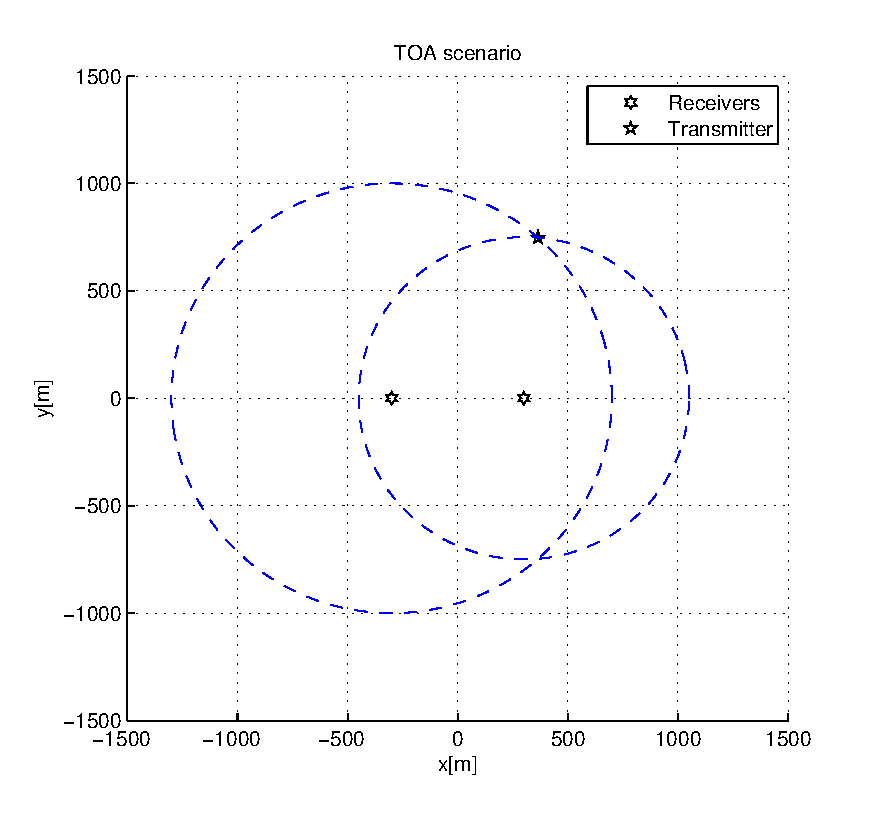
\includegraphics[scale=0.7]{TOA_scenario.eps}
\end{center}
\caption[TOA Scenario]{TOA Scenario. Two stationary receivers are located in (-300,0) and (300,0). The estimated TOA for each receiver forms a circle of possible transmitter locations around each receiver. The two circles intersect at two points that are the two possible transmitter locations. Using a-priori information regarding the position of the transmitter, the two possible transmitter positions can be reduced to a single estimated position.}
\label{fig:TOA_scenario}
\end{figure}

In TDOA based methods, each TDOA measurement locates the transmitter on a hyperbola of possible transmitter locations. At least another TDOA measurement is necessary in order to locate the transmitter at several points of intersection of the two hyperbolas. Using a-priori information about the transmitter location the several possible points can be reduced to a single solution.
Again, as additional receivers are added, the hyperboloids will not intersect in one point because of noisy measurements and errors, and the need to use estimation methods arises.
Chan and Ho \cite{chan_and_ho} suggested a simple and efficient estimator for hyperbolic location systems, and Chestnut \cite{chestnut} suggested a method for estimating the position of a stationary transmitter based on TDOA measurements and analysed its performance.\\

Figure (\ref{fig:TDOA_scenario}) shows an example of the TDOA based scenario: Two receivers are located at (-300,0) and (300,0). The TDOA measurement of this pair of receivers forms a hyperbola of possible transmitter positions. At least one more receiver is necessary in order to determine the position the transmitter.

\begin{figure}
\begin{center}
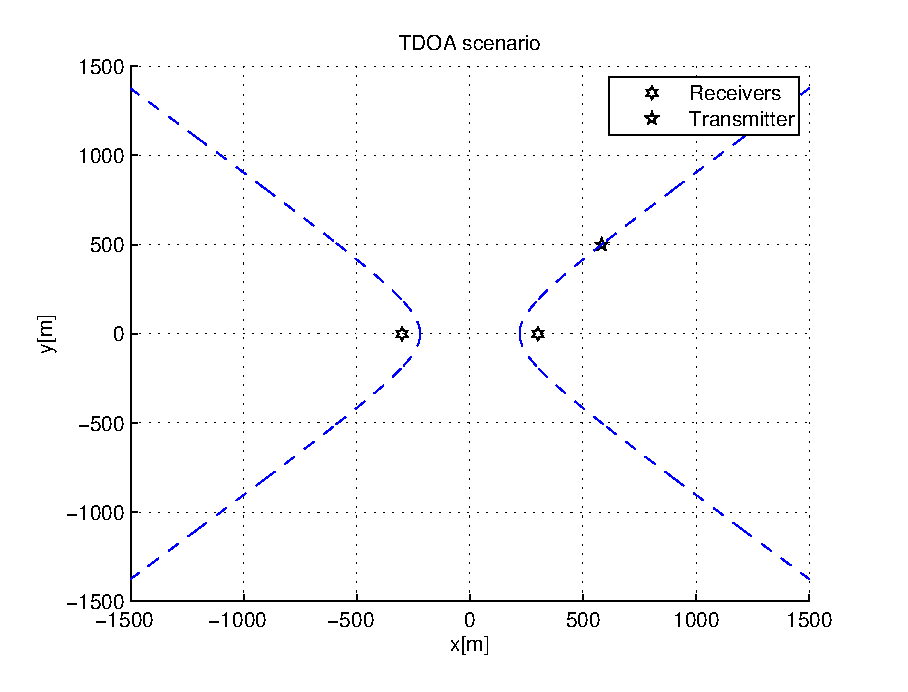
\includegraphics[scale=0.7]{TDOA_scenario.eps}
\end{center}
\caption{TDOA Scenario. Two receivers are located at (-300,0) and (300,0). The TDOA measurement of this pair of receivers forms a hyperbola of possible transmitter positions. At least one more receiver is necessary in order to determine the position the transmitter.}
\label{fig:TDOA_scenario}
\end{figure}

It is interesting to mention that the TDOA estimated in a single interval contains no information regarding the velocity of the transmitter. Thus, the velocity of the transmitter cannot be estimated using the TDOA measurements.\\

There are many suggested methods for estimating the position of a transmitter based on TDOA measurements. We will shortly introduce the application of the Weighted-Least-Squares(WLS) method, because of its relative simplicity, and only to acquire some intuition.\\

In the first step of the method introduced, the difference in the time-of-arrival is estimated for every pair of receivers, so that the matrix $\mathbf{\hat{T}}$ is estimated. The $i,j$-th element of the matrix $\mathbf{\hat{T}}$ is the time-of-arrival difference between the $i$-th and the $j$-th receivers.\\


For the transmitter position $\vec{p}$, and receivers positions $\vec{p_\ell}$, the expected $\mathbf{T(\vec{p}})$ matrix can be calculated:
\begin{equation}
T(\vec{p})_{i,j} = \frac{1}{C}\|\vec{p_i}-\vec{p}\|-\frac{1}{C}\|\vec{p_j}-\vec{p}\|
\end{equation}
The $i$,$j$-th element of $\mathbf{T(\vec{p}})$ is the expected TDOA between the $i$-th and the $j$-th receivers, if the transmitter position is $\vec{p}$.\\

A WLS TDOA cost function can then be defined as:
\begin{equation}
C_{\text{TDOA}}(\vec{p}) = \sum_{i=1}^L \sum_{j=1}^L w_{i,j}(T(\vec{p})_{i,j}-\hat{T}_{i,j})^2
\end{equation}
Where $w_{i,j}$ is the $i$,$j$-th element of the weights matrix $W$.

The WLS estimator for the position is the position $\hat{\vec{p}}$ for which the value of the WLS cost function is minimal. 
Therefore:
\begin{equation}
\hat{\vec{p}} = \text{argmin}_{\vec{p}}C_{\text{TDOA}}(\vec{p})
\end{equation}

The Known-Signals FIM related to the TOA estimation of the $\ell$-th signal is:
\begin{equation}
\text{FIM}_{\ell,\ell} = \frac{2}{\sigma_\ell^2}\left\|\frac{\partial \mathbf{m_\ell}}{\partial T_\ell}\right\|^2
\end{equation}
Where we assumed that the noise in the receivers is Gaussian i.i.d, independent between the receivers, with variance $\sigma_\ell^2$ in each receiver. The data vector $\mathbf{m_\ell}$ is the time shifted known signal, as was received in the $\ell$-th receiver if there was no noise.\\
Because $\mathbf{m_l}$ depends only on the time delay of the $\ell$-th receiver, the FIM is diagonal.
Thus:
\begin{equation}
\text{CRB}_\ell = \frac{\sigma_\ell^2}{2\left\|\frac{\partial \mathbf{m_\ell}}{\partial T_\ell}\right\|^2}
\end{equation}
So that:
\begin{equation}
\text{VAR}(\text{TOA}_\ell) \geq \frac{\sigma_\ell^2}{2\left\|\frac{\partial \mathbf{m_\ell}}{\partial T_\ell}\right\|^2}
\end{equation}
Assuming that the TOA measurements were taken using an efficient estimator, the CRB can be used to determine the weights matrix $W$.

\subsection{FOA and FDOA Based Passive Geolocation}
In the following subsection we discuss the methods to geolocate a transmitter using FOA and FDOA based methods.\\

When the transmitter is moving with a relative radial velocity to the receiver, a frequency shift of the transmitted signal is caused due to the Doppler effect.\\
Similarly to the TDOA based methods, the exact original transmitted frequency is usually unknown, and requires measurement of the FDOA between each pair of receivers.
The methods that use these measurements are sometimes also referred to as DD.\\

FOA and FDOA measurements contain information on both the position and velocity of the transmitter, unlike TDOA measurements that only contain information about the position of the transmitter. \\
Nevertheless, in order to acquire the FDOA measurements, a relative motion of the transmitter and the receivers is necessary, limiting the scenarios applicable for this method.\\

A simple, intuitive geometrical interpretation of the FDOA estimation methods is less direct, but is possible if we make a few assumptions and limit the discussion to simple scenarios. We present here two simple examples: Positioning of a stationary transmitter, transmitting a known frequency, using a moving receiver, and positioning of a stationary transmitter, transmitting an unknown frequency, using 2 moving receivers.\\

We start by describing the known transmitted frequency scenario: Consider a scenario in which the transmitter is stationary and a receiver is moving in a constant known velocity $\vec{v}$, transmitting a signal with a known frequency. The Doppler frequency shift will be proportional to the carrier frequency $F_c$ and to the relative radial velocity $\|\vec{v}\|cos\theta$, where $\theta$ is the angle between the velocity and the line connecting the transmitter and the receiver, as can be seen in figure (\ref{fig:DOP_scenario}). Because the transmitted frequency is known, the Doppler shift can be easily estimated. Since $\vec{v}$ and $F_c$ are known, $cos\theta$ can be estimated from the estimated Doppler shift, and 2 lines on which the transmitter is located are defined.\\
Additional receivers create additional lines that the transmitter lies in their spatial intersection.\\

\begin{figure}
\begin{center}
\includegraphics[scale=0.5]{DOP_scenario.eps}
\end{center}
\caption{FOA based geolocation scenario. A receiver is moving at velocity $\vec{v}$, forming an angle $\theta$ with the line connecting the positions of the receiver and the transmitter.}
\label{fig:DOP_scenario}
\end{figure}


In the case where the transmitted frequency is unknown, the Doppler shift cannot be estimated directly, and only the FDOA between pairs of receivers can be estimated. Figure (\ref{fig:FDOA_scenario}) describes a scenario in which two receivers are moving in velocities $\vec{v_1}$ and $\vec{v_2}$, forming the angles $\theta_1$ and $\theta_2$ with the lines connecting their position and the position of the transmitter. The lines connecting the position of the receivers and the position of the transmitter form the angles $\alpha_1$ and $\alpha_2$ with the $x$-axis. The FDOA between the two receivers is denoted by $\Delta f_{1,2}$.

We define the difference between the radial velocity of the receivers in relation to the transmitter by $\Delta v_{r,1,2}$ as follows:
\begin{equation}
\label{eq:Delta_v_def}
\Delta v_{r,1,2} \triangleq \|\vec{v_1}\|\text{cos}\theta_1 - \|\vec{v_2}\|\text{cos}\theta_2
\end{equation}
And then $\Delta f_{1,2}$ can be expressed as:
\begin{equation}
\label{eq:Delta_f_12}
\Delta f_{1,2}= \frac{F_c}{c} \Delta v_{r,1,2}
\end{equation}

Assuming that $\theta_2$ is known, by rearranging equation (\ref{eq:Delta_v_def}):
\begin{equation}
\label{eq:cos_theta_1}
\text{cos}\theta_1 = \frac{\Delta v_{r,1,2} + \|\vec{v_2}\|\text{cos}\theta_2}{\|\vec{v_1}\|}
\end{equation}

By rearranging equation (\ref{eq:Delta_f_12}) and substituting into (\ref{eq:cos_theta_1}) we get:
\begin{equation}
\text{cos}\theta_1 = \frac{\frac{c}{F_c}\Delta f_{1,2} + \|\vec{v_2}\|\text{cos}\theta_2}{\|\vec{v_1}\|}
\end{equation}

And so $\theta_1$ can be expressed as a function of $\theta_2$:

\begin{equation}
\label{eq:FDOA_curve}
\theta_1(\theta_2) = \text{arcos}\frac{\frac{c}{F_c}\Delta f_{1,2} + \|\vec{v_2}\|\text{cos}\theta_2}{\|\vec{v_1}\|}
\end{equation}

Equation (\ref{eq:FDOA_curve}) above describes a constant FDOA curve. The curve is defined by the known receiver velocities, and by the estimated FDOA. Every point on the curve is a possible transmitter position. Adding another receiver creates two more constant FDOA curves that the receiver lies in their intersection.

Figure (\ref{fig:FDOA_scenario_example}) shows an example of a constant FDOA curve. Two receivers are located at $(-300,0)$ and $(300,0)$ and moving with a $10[m/s]$ velocity in the positive $x$-axis direction, and the transmitter is located at $(1000,500)$.

\begin{figure}
\begin{center}
\includegraphics[scale=0.5]{FDOA_scenario.eps}
\end{center}
\caption{FDOA based geolocation scenario. Two receivers are moving in velocities $\vec{v_1}$ and $\vec{v_2}$, forming the angles $\theta_1$ and $\theta_2$ with the lines connecting their position and the position of the transmitter. The lines connecting the position of the receivers and the position of the transmitter form the angles $\alpha_1$ and $\alpha_2$ with the $x$-axis.}
\label{fig:FDOA_scenario}
\end{figure}

\begin{figure}
\begin{center}
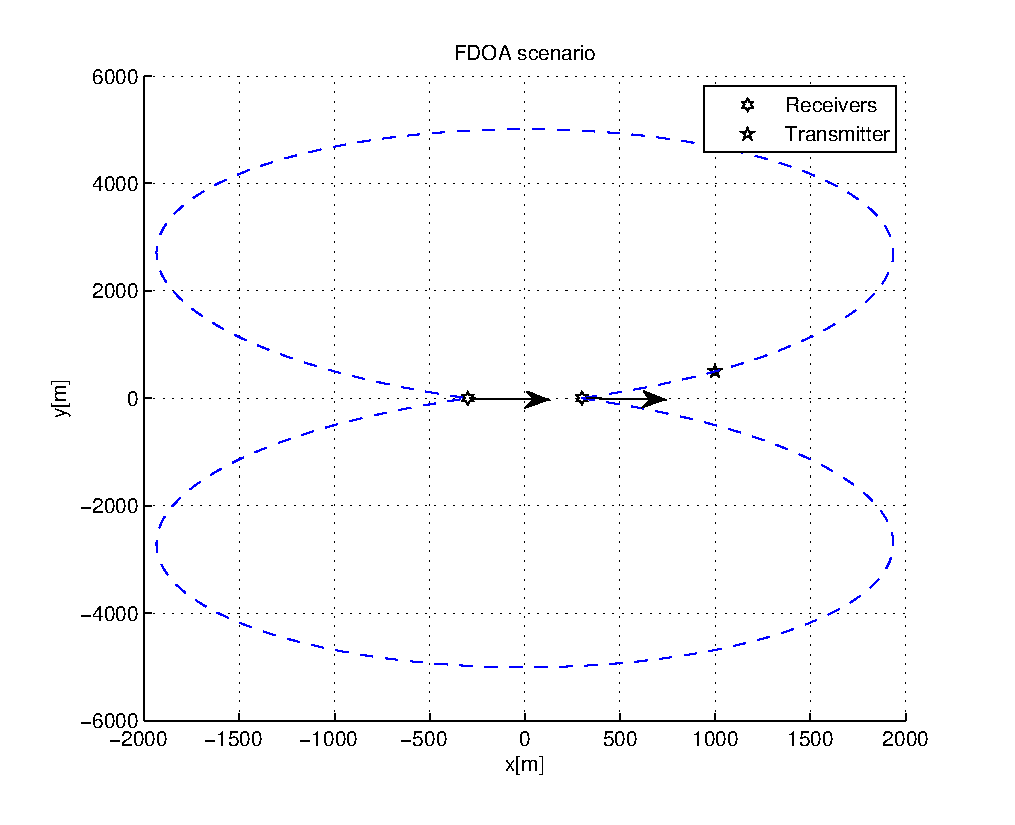
\includegraphics[scale=0.7]{FDOA_scenario_example.eps}
\end{center}
\caption{Constant FDOA curve example. Two receivers are located at $(-300,0)$ and $(300,0)$, moving with a $10[m/s]$ velocity in the positive $x$-axis direction. The transmitter is located at $(1000,500)$.}
\label{fig:FDOA_scenario_example}
\end{figure}

Just in order to acquire some understanding of FDOA based geolocation methods, we introduce a simple WLS estimation method.\\

In the first step of the method introduced, the difference in the frequency-of-arrival is estimated for every pair of receivers, so that the matrix $\hat{F}$ is estimated. The $i,j$-th element of the matrix $\hat{F}$ is the frequency-of-arrival difference between the $i$-th and the $j$-th receiver.\\

For transmitter position and velocity $(\vec{p},\vec{v})$, the expected $F(\vec{p},\vec{v})$ matrix can be calculated:
\begin{equation}
F(\vec{p},\vec{v})_{i,j} = -\frac{F_c}{c}\frac{(\vec{v}-\vec{v_i})(\vec{p}-\vec{p_i})}{|\vec{p}-\vec{p_i}|}+\frac{F_c}{c}\frac{(\vec{v}-\vec{v_j})(\vec{p}-\vec{p_j})}{|\vec{p}-\vec{p_j}|}
\end{equation}
Where $F_c$ is the carrier frequency of the signal, $c$ is the propagation speed of the signal, $\vec{v}$ is the velocity of the transmitter and $\vec{v_i}$ is the velocity of the $i$-th receiver.\\

A WLS cost function can then be defined as:

\begin{equation}
C_{\text{FDOA}}(\vec{p},\vec{v}) = \sum_{i=1}^L \sum_{j=1}^L w_{i,j}(F(\vec{p},\vec{v})_{i,j}-\hat{F}_{i,j})^2
\end{equation}

Where $w_{i,j}$ is the $i$,$j$-th element of the weight matrix $W$.
The WLS estimator for the position and velocity of the transmitter is the position and velocity that minimize the cost function:

\begin{equation}
(\hat{\vec{p}},\hat{\vec{v}}) = \text{argmin}_{(\vec{p},\vec{v})}C_{\text{FDOA}}(\vec{p},\vec{v})
\end{equation}

As opposed to the TDOA estimator, we can see that the FDOA estimate depends both on the position and on the velocity of the transmitter. Thus, both the position and velocity of the transmitter can be estimated using the FDOA measurements.\\

The Known-Signals Fischer information matrix related to the FDOA estimation of the $\ell$-th signal is:

\begin{equation}
\text{FIM}_\ell = \frac{2}{\sigma_\ell^2}\left\|\frac{\partial \mathbf{m_\ell}}{\partial f_\ell}\right\|^2
\end{equation}

Where $f_\ell$ is the frequency shift caused by the Doppler effect. We used the assumption that the noise in the receivers is Gaussian i.i.d, independent between the receivers, with variance $\sigma_\ell^2$ in each receiver. The data vector $\mathbf{m_\ell}$ is the frequency shifted known signal, as was received in the $\ell$-th receiver if there was no noise.\\
Because $\mathbf{m_l}$ depends only on the frequency shift of the $\ell$-th receiver, the FIM is diagonal.
Thus:

\begin{equation}
\text{VAR}(\text{FOA}_\ell)\geq\text{CRB}_\ell = \frac{\sigma_\ell^2}{2\left\|\frac{\partial \mathbf{m_\ell}}{\partial f_\ell}\right\|^2}
\end{equation}

Assuming that the FDOA measurements were taken using an efficient estimator, the CRB can be used to determine the weights matrix $W$.

\subsection{TDOA-FDOA Based Passive Geolocation}
\label{subsec:tdoa_fdoa}
We can easily combine the two methods suggested above using the weighted least squares (WLS) method.
If we assume that the TDOA and FDOA estimations were performed by an efficient estimator, we can use the calculated CRB for TDOA and FDOA to define the weight matrices $W_T$ and $W_F$ for the TDOA measurements and for the FDOA measurements respectively.
Then, the measurements can be combined in the following cost function:
\begin{equation}
C_{TF}(\vec{p},\vec{v}) = \sum_{i=1}^L \sum_{j=1}^L {w_T}_{i,j}(T(\vec{p})_{i,j}-\hat{T}_{i,j})^2+ {w_F}_{i,j}(F(\vec{p},\vec{v})_{i,j}-\hat{F}_{i,j})^2
\end{equation}
Where ${w_T}_{i,j}$ and ${w_F}_{i,j}$ are the $i$,$j$-th elments of the TDOA and FDOA weight matrices respectively.
The estimated position and velocity are the position and velocity that minimize the cost function:
\begin{equation}
(\hat{\vec{p}},\hat{\vec{v}}) = \text{argmin}_{(\vec{p},\vec{v})}C_{TF}(\vec{p},\vec{v})
\end{equation}

\section{DPD Algorithm Concepts}
In this section we introduce the main ideas and concepts behind the DPD algorithm \cite{dpd}.\\

Most common methods consist of two steps. The first step is to estimate a certain parameter of the
SOI, such as TDOA or FDOA. \\
The second step is to use the parameter estimated at each of the receivers, or receivers pairs, to estimate the location of the transmitter.\\
It is important to note that the estimation of the SOI parameters is done independently in each receiver or pair of receivers, so that the information used in each of the estimations is partial, consists only on the samples collected by its own antennas and does not take into consideration that all of the received signals have a common origin.\\
The DPD algorithm uses exactly the same data used in conventional methods, but it skips the first step of parameter estimation. All of the samples are collected at a central base station, and the location of the transmitter is estimated using all of the samples at once, without making any intermediate estimations.\\

The DPD algorithm advantages are mainly better performance over conventional methods using the same data and conceptual simplicity. The DPD algorithm main drawbacks are its computational complexity and the need for high band-width communication between the receivers and the central processing station in order to transfer the entire sampled signals from the receivers to the processing station.\\

The original DPD algorithm\cite{dpd} has been developed in recent years, and is now related to a family of algorithms, each of which related to a different scenario.
The original DPD algorithm \cite{dpd} assume a static scenario, in which both the transmitters and the receivers are stationary. The algorithm uses the time delays and the sensors spatial response function in order to locate multiple radio transmitters.\\

In \cite{dop_dpd_nb} a direct algorithm for the location a stationary narrow-band transmitter using an array of moving receivers is presented. The algorithm assumes that the signal is narrow band, so that the envelope of the received signal is identical in all of the receivers. The different Doppler shifts observed by the receivers are used in order to localize the transmitter. A likelihood cost function is derived, and grid-search is suggested in order to find the maximum-likelihood estimation.\\

In \cite{dop_dpd_wb} the direct algorithm is extended for locating a stationary wide-band transmitter using an array of moving receivers. This algorithm takes advantage on both the different Doppler shifts and time-delays observed by the different receivers.\\

All of the direct methods suggested above show better performance than conventional methods using the same data. The direct methods show better performance especially in low-SNR scenarios. 

In this work, we present a direct passive location algorithm for a moving transmitter using a stationary array of receivers.

\section{Outline}
\begin{itemize}
\item \textbf{Chapter 1} (this chapter) consists of an introduction to this work and of a literature survey.
\item \textbf{Chapter 2} presents the problem formulation and the derived ML estimator. The chapter handles the scenarios in which the transmitted signal is known or unknown, wide-band or narrow-band.
\item \textbf{Chapter 3} explores the characteristics of the known-signals cost function $L_2$. The function is explored in order to acquire some intuition on its behaviour, and its derivatives are developed in order to be used by gradient-based search methods.
\item \textbf{Chpater 4} suggests several possible location algorithms for different scenarios. Grid search algorithms and gradient-based algorithms are suggested. For the scenario in which the transmitter is tracked, a Kalman-filter based approach is suggested.
\item \textbf{Chapter 5} develops the known-signals Cramer-Rao lower bound of the problem.
\item \textbf{Chapter 6} presents the simulation results of several different scenarios. The results of the suggested algorithm are compared to the Cramer-Rao lower bound, and to conventional methods.
\end{itemize}